% !TEX root = manuscript.tex

\chapter*{Annexes}
\addcontentsline{toc}{chapter}{Annexes} 

\section*{Annexe 3}
\label{sec:annexe3}
\begin{figure}[H]
\centering
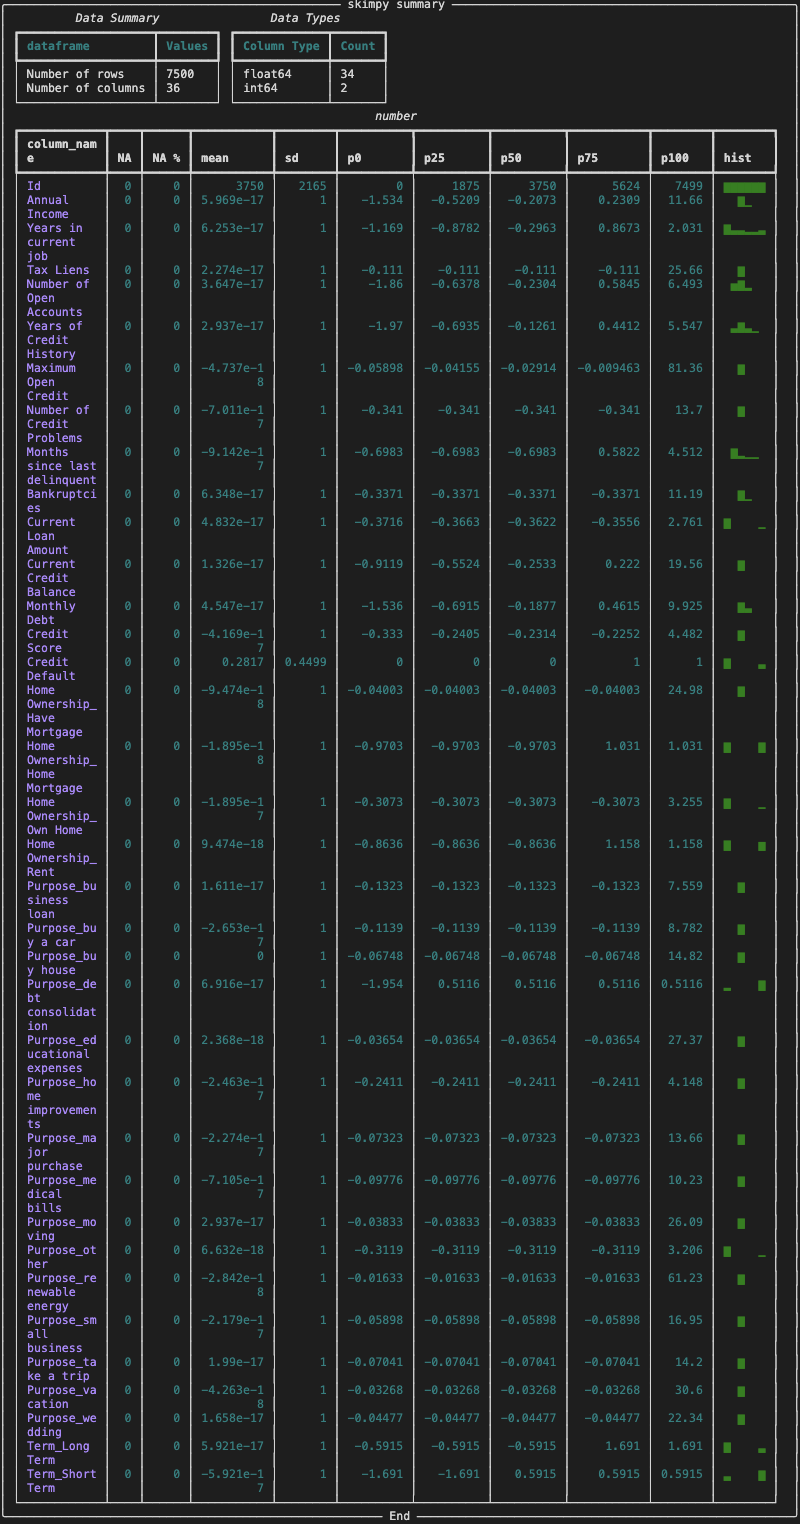
\includegraphics[width=0.5\textwidth]{figures/Annexe3.png}
\caption{Résumé Statistique descriptive train.}
\label{fig:annexe3}
\end{figure}

\section*{Annexe 4}
\label{sec:annexe4}
\begin{figure}[H]
\centering
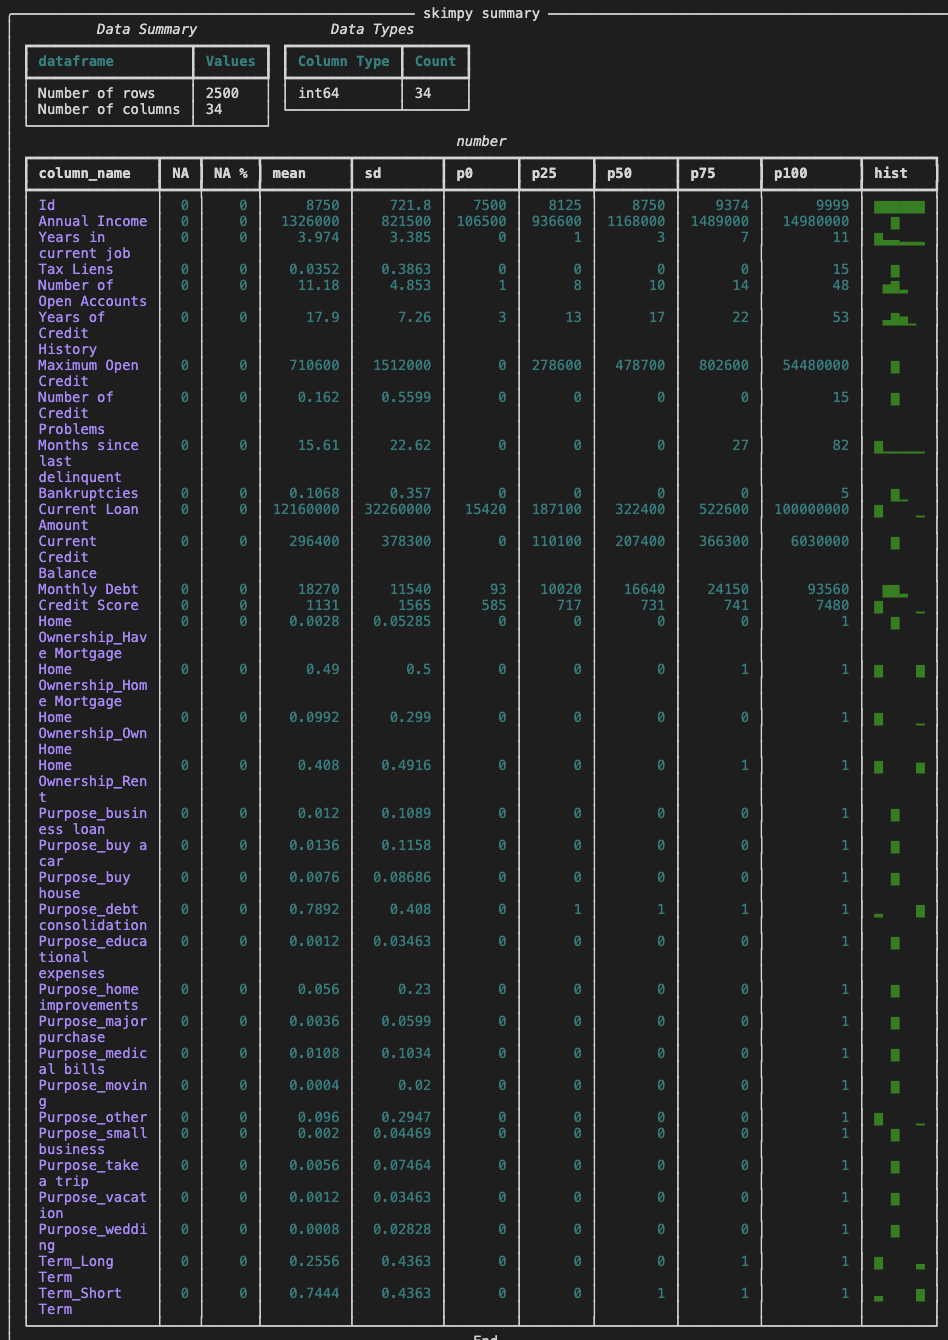
\includegraphics[width=0.5\textwidth]{figures/Annexe4.png}
\caption{Résumé Statistique descriptive jeu test.}
\label{fig:annexe4}
\end{figure}

\section*{Annexe 5}
\label{sec:annexe5}
\begin{figure}[H]
\centering
\includegraphics[width=0.5\textwidth]{figures/MatriceArbre.png}
\caption{Matrice de confusion Arbre de décision.}
\label{fig:annexe5}
\end{figure}


\begin{figure}[H]
\centering
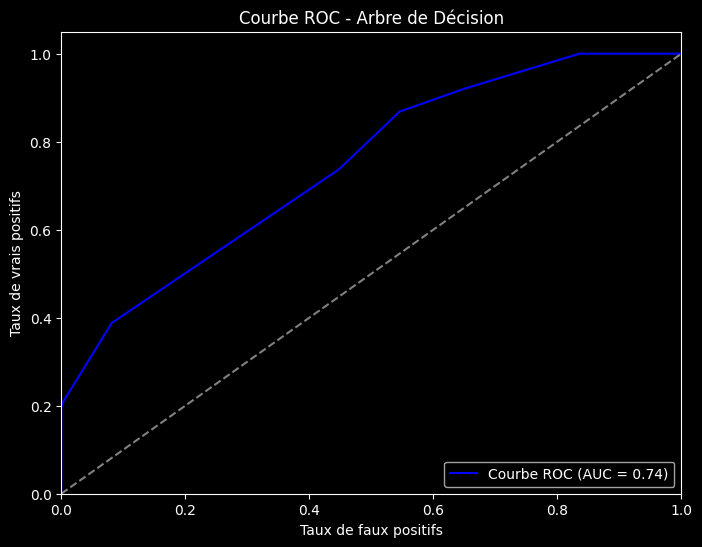
\includegraphics[width=0.5\textwidth]{figures/ROCArbre.png}
\caption{Courbe de ROC Arbre de décision.}
\end{figure}


\section*{Annexe 6}
\label{sec:annexe6}
\begin{figure}[H]
\centering
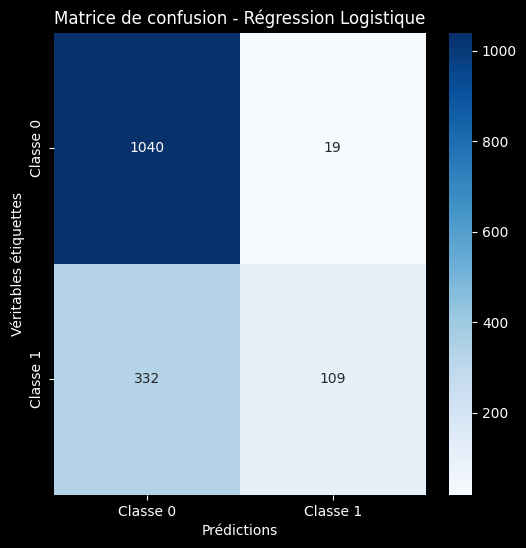
\includegraphics[width=0.5\textwidth]{figures/MatriceRL.png}
\caption{Matrice de confusion Régression logistique.}
\label{fig:annexe6}
\end{figure}


\begin{figure}[H]
\centering
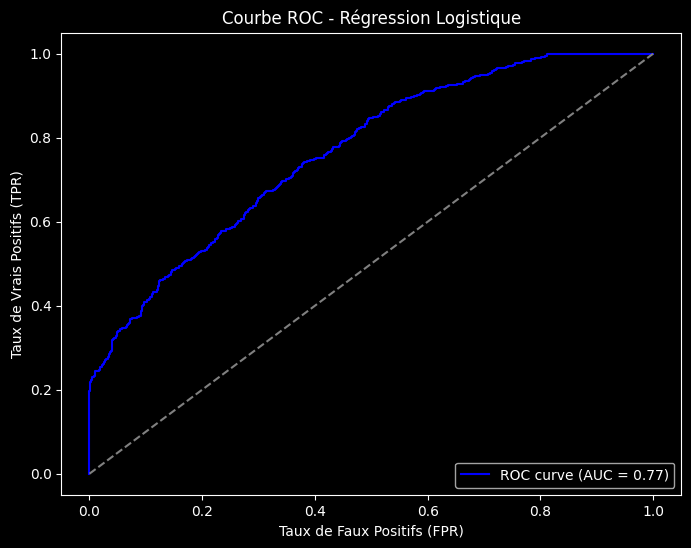
\includegraphics[width=0.5\textwidth]{figures/ROCRL.png}
\caption{Courbe de ROC Régression Logistique.}
\end{figure}

\section*{Annexe 7}
\label{sec:annexe7}
\begin{figure}[H]
\centering
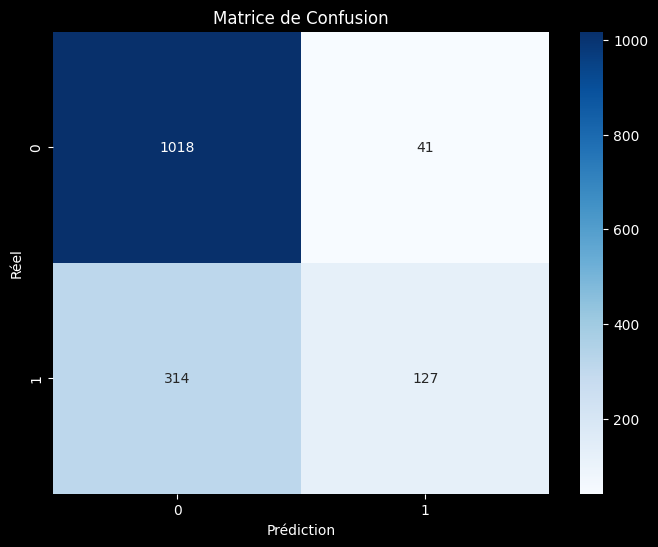
\includegraphics[width=0.5\textwidth]{figures/MatriceFoAl.png}
\caption{Matrice de confusion Forêt Aléatoire.}
\label{fig:annexe7}
\end{figure}


\begin{figure}[H]
\centering
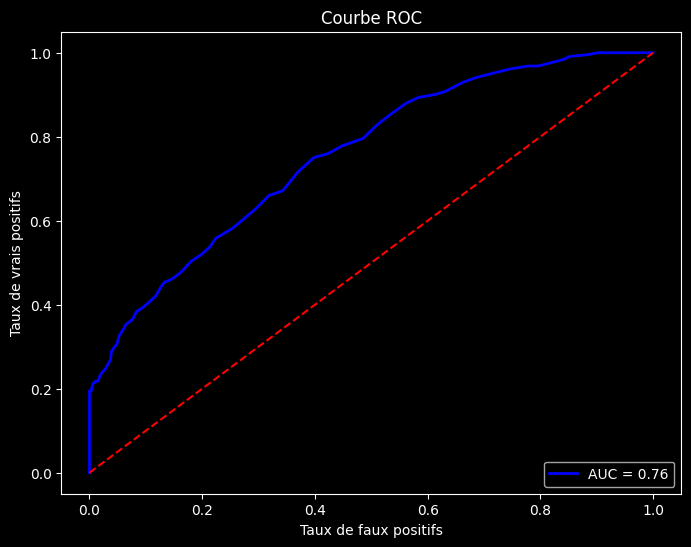
\includegraphics[width=0.5\textwidth]{figures/ROCAL.png}
\caption{Courbe de ROC Forêt Aléatoire}
\end{figure}

\section*{Annexe 8}
\label{sec:annexe8}
\begin{figure}[H]
\centering
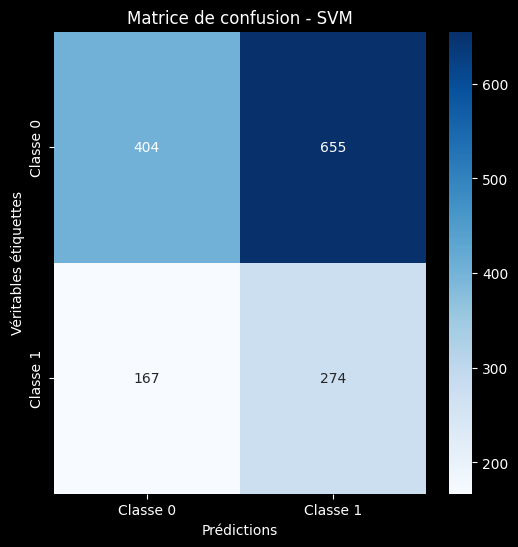
\includegraphics[width=0.5\textwidth]{figures/MatriceSVM.png}
\caption{Matrice de confusion SVM.}
\label{fig:annexe8}
\end{figure}


\begin{figure}[H]
\centering
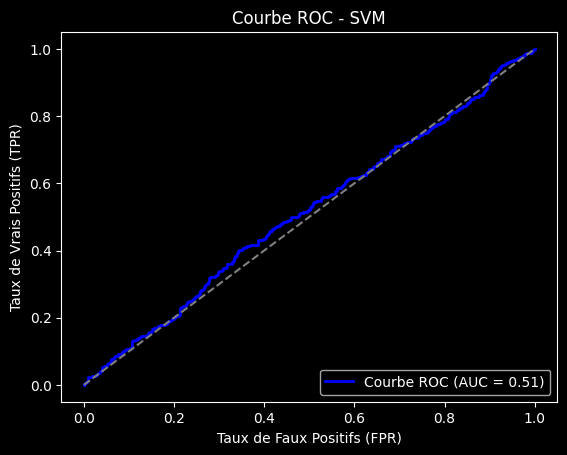
\includegraphics[width=0.5\textwidth]{figures/ROCSVM.png}
\caption{Courbe de ROC SVM.}
\end{figure}

\section*{Annexe 9}
\label{sec:annexe9}
\begin{figure}[H]
\centering
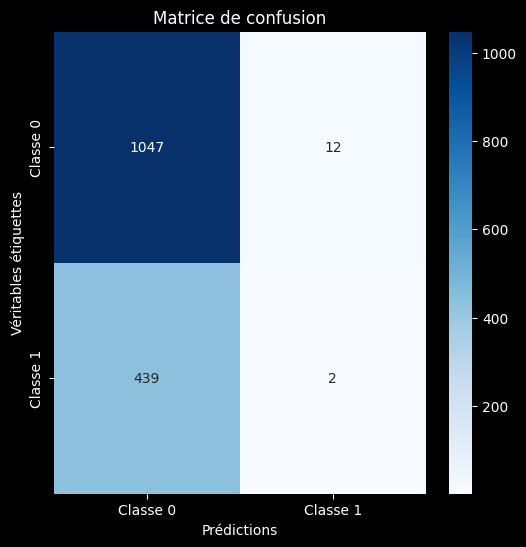
\includegraphics[width=0.5\textwidth]{figures/MatriceKNN.png}
\caption{Matrice de confusion KNN.}
\label{fig:annexe9}
\end{figure}


\begin{figure}[H]
\centering
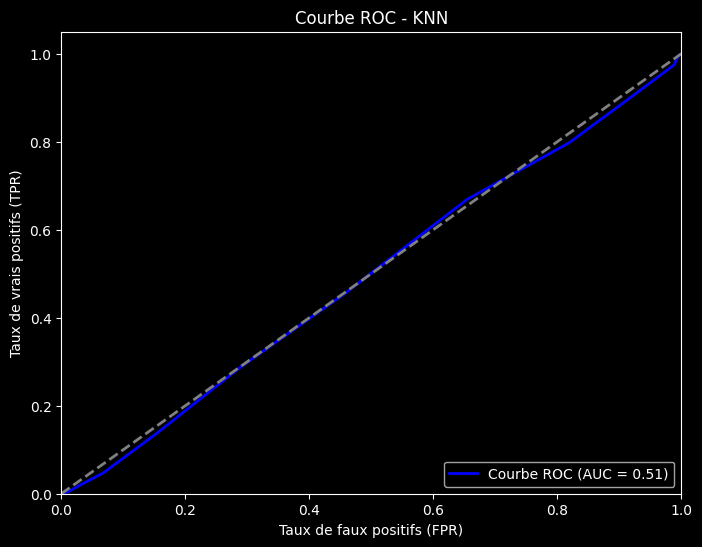
\includegraphics[width=0.5\textwidth]{figures/ROCKNN.png}
\caption{Courbe de ROC KNN.}
\end{figure}
\section*{Annexe 10}
\label{sec:annexe10}
\begin{figure}[H]
\centering
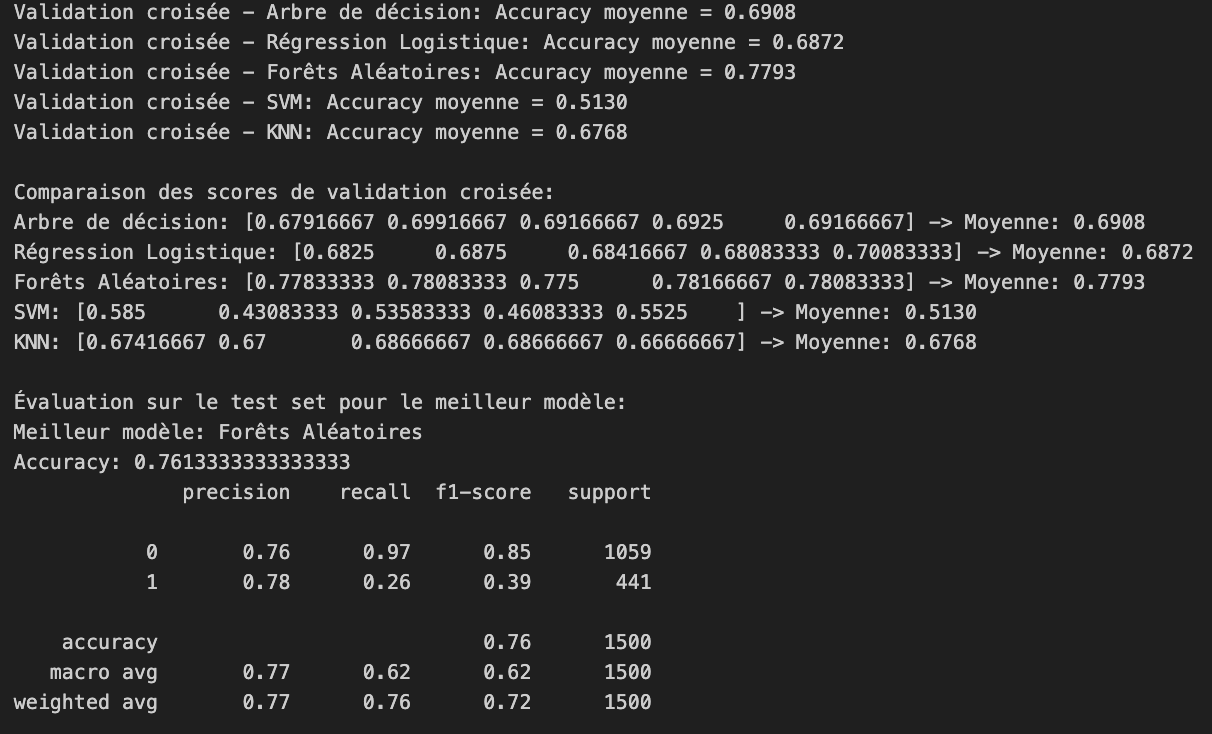
\includegraphics[width=0.5\textwidth]{figures/Annexe10.png}
\caption{Métrique Validation Forêt Aléatoire.}
\label{fig:annexe10}
\end{figure}

\begin{figure}[H]
\centering
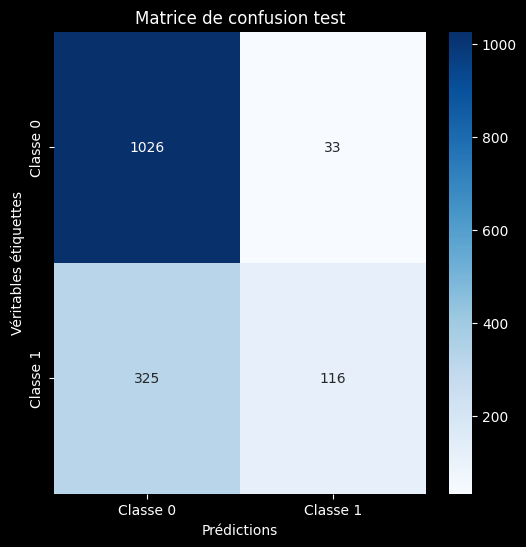
\includegraphics[width=0.5\textwidth]{figures/MatriceVC1.png}
\caption{Matrice de validation croisée Forêt Aléatoire.}
\end{figure}


\section*{Annexe 11}
\label{sec:annexe11}
\begin{figure}[H]
\centering
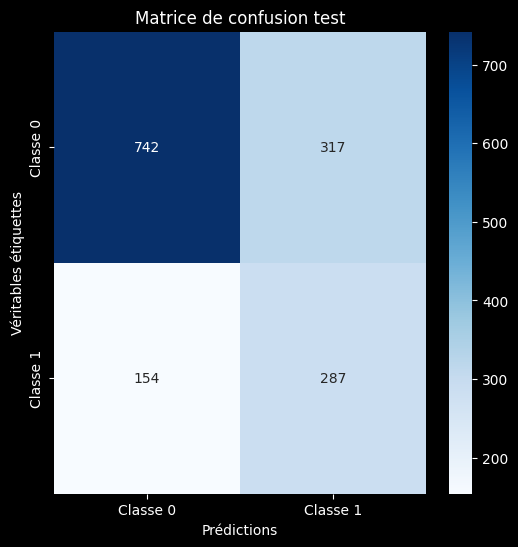
\includegraphics[width=0.5\textwidth]{figures/MatriceValANNEXE11.png}
\caption{Matrice de validation croisée Régression Logistique.}
\label{fig:annexe11}
\end{figure}
